\documentclass[a4paper,10pt]{article}

% рисунки
\usepackage{graphicx}

\usepackage[T2A]{fontenc}
\usepackage[utf8]{inputenc}
\usepackage[english,russian]{babel}

\RequirePackage{caption}
\DeclareCaptionLabelSeparator{defffis}{ — }
\captionsetup{justification=centering,labelsep=defffis}

\usepackage{caption} \captionsetup[table]{labelsep=endash,justification=justified,singlelinecheck=false,font=normalsize}

\usepackage{amsmath,amsfonts,amssymb,amsthm,mathtools}



\begin{document}
  
\begin{center}
  \section*{Лабораторная работа №3.2.2 \\Резонанс напряжений в последовательном контуре\\Джокер Бэтмен, Б02-000, 18.09.2021}
\end{center}  

\vspace{5mm}
\section*{Введение}

\begin{flushleft}
  \textbf{Цель работы:} исследование резонанса напряжений в последовательном колебательном контуре с изменяемой ёмкостью, получение амплитудно-частотных и фазово-частотных характеристик, определение основных параметров контура.

\end{flushleft}

\begin{flushleft}
  \textbf{В работе используются:} генератор сигналов, источник напряжения, нагрузкой которого является последовательный колебательный контур с переменной ёмкостью, двухканальный осциллограф, цифровые вольтметры.

\end{flushleft}

\section*{Теоретическая справка}

В теории переменных токов напряжения и токи принято выражать комплексными числами. Модуль комплексного числа равен эффективному значению напряжения (или тока), а фаза -- сдвигу фаз, измеренному по отношению к какому-либо одному напряжению или току, принятому в качестве опорного. Параметры основных элементов цепи задаются их импедансами, т.е. тоже некоторыми комплексными числами.

Рассмотрим электрическую цепь, состоящую из резистора $R$ и катушки индуктивности $L$ с импедансами $Z_L=r_L+i\Omega L$, последовательно подключенных к внешнему источнику, ЭДС которого меняется по синусоидальному закону с частотой $\Omega$.

Обозначим через $U_R$ напряжение на резисторе, через $U_L$ -- напряжение на катушке и через $U_{R+L}$ -- суммарное напряжение на катушке и на резисторе. Для этих напряжений справедливы комплексные соотношения:\[\hat{U}_R=\hat{I}R,\ \hat{U}_L=\hat{I}\left(r_L+i\Omega L\right),\ \hat{U}_{R+L}=\hat{I}\left(R+r_L+i\Omega L\right).\]Напомним, что здесь $r_L$ -- активное сопротивление катушки, которое характеризует суммарные потери энергии в катушке, в том числе потери в её ферромагнитном сердечнике.

Переходя к модулям и фазам токов и напряжений, найдём:
\begin{flalign*}
& U_R=IR, && \tg{\psi_1}=0; && \\
& U_L=I\sqrt{r_L^2+\left(\Omega L\right)^2}, && \tg{\psi_2}=\frac{\Omega L}{r_L}; && \\
& U_{R+L}=I\sqrt{\left(R+r_L\right)^2+\left(\Omega L\right)^2}, && \tg{\psi_3}=\frac{\Omega L}{R+r_L}. &&
\end{flalign*}
В этих формулах $U$ и $I$ обозначают эффективные значения напряжений и токов (показания приборов).

Измеряя с помощью трёх вольтметров значения $U_R$, $U_L$ и $U_{R+L}$ и зная сопротивление резистора $R$, нетрудно вычислить силу тока в цепи, активное сопротивление катушки $r_L$, её индуктивность $L$, мощность $P_L$, выделяемую на катушке, и сдвиг фаз между током и напряжением на катушке.

Рассчитаем мощность переменного тока, выделяемую на катушке. Мгновенное значение мощности равно\[P=U(t)I(t).\]Средняя мощность за период $T$ определяется формулой\[P=\frac{1}{T}\int^T_0U(t)I(t)\text{d}t.\]Полагая $I(t)=I\sqrt2\cos{\left(\Omega t\right)},\ U(t)=U\sqrt2\cos{\left(\Omega t+\psi\right)}$, получим после интегрирования:\[\bar{P}_L=U_LI\cos{\psi}=I^2r_L.\]Средняя мощность, выделяющаяся в катушке самоиндукции, определяется, таким образом, действительной частью её импеданса.

Активное сопротивление катушки $r_L$ можно определить, если включить её в последовальный колебательный контур с известными параметрами -- сопротивлением $R$ и ёмкостью $C$. В контуре, настроенном в резонанс на частоту $\Omega$ внешнего источника (собственная частота контура и внешняя частота совпадают: $\omega=\Omega$), реактивные сопротивления индуктивности и ёмкости равны:\[\omega_0L=\frac{1}{\omega_0C}.\]Определив каким-либо экспериментальным способом добротность $Q$ этого контура, можно рассчитать полное сопротивление контура $R_{\Sigma}$ в резонансе, поскольку\[Q=\frac{\omega_0L}{R_{\Sigma}}=\frac{1}{\omega_0CR_{\Sigma}}.\]Резонансное сопротивление контура $R_{\Sigma}$ включает в себя известное сопротивление резистора $R$ и активное сопротивление катушки $r_L$:\[R_{\Sigma}=R+r_L.\]

\section*{Экспериментальная установка}

Схема установки для исследования закона Ома в цепи переменного тока представлена на рис. \Ref{Device}. Цепь, состоящая из резистора $R_1\approx100~\Omega$ и катушки $L$ с выдвижным сердечником подключена к трансформатору, выходное напряжение которого можно изменять от 0  до 127 В. Напряжения на каждом из элементов и суммарное напряжеие цепи измеряются тремя вольтметрами: $V_R$, $V_L$ и $V_{R+L}$. Амперметр $A$ измеряет ток в цепи, а ваттметр $P$ -- мощность, выделяющуюся на катушке.

\begin{figure}[h]
	\centering
	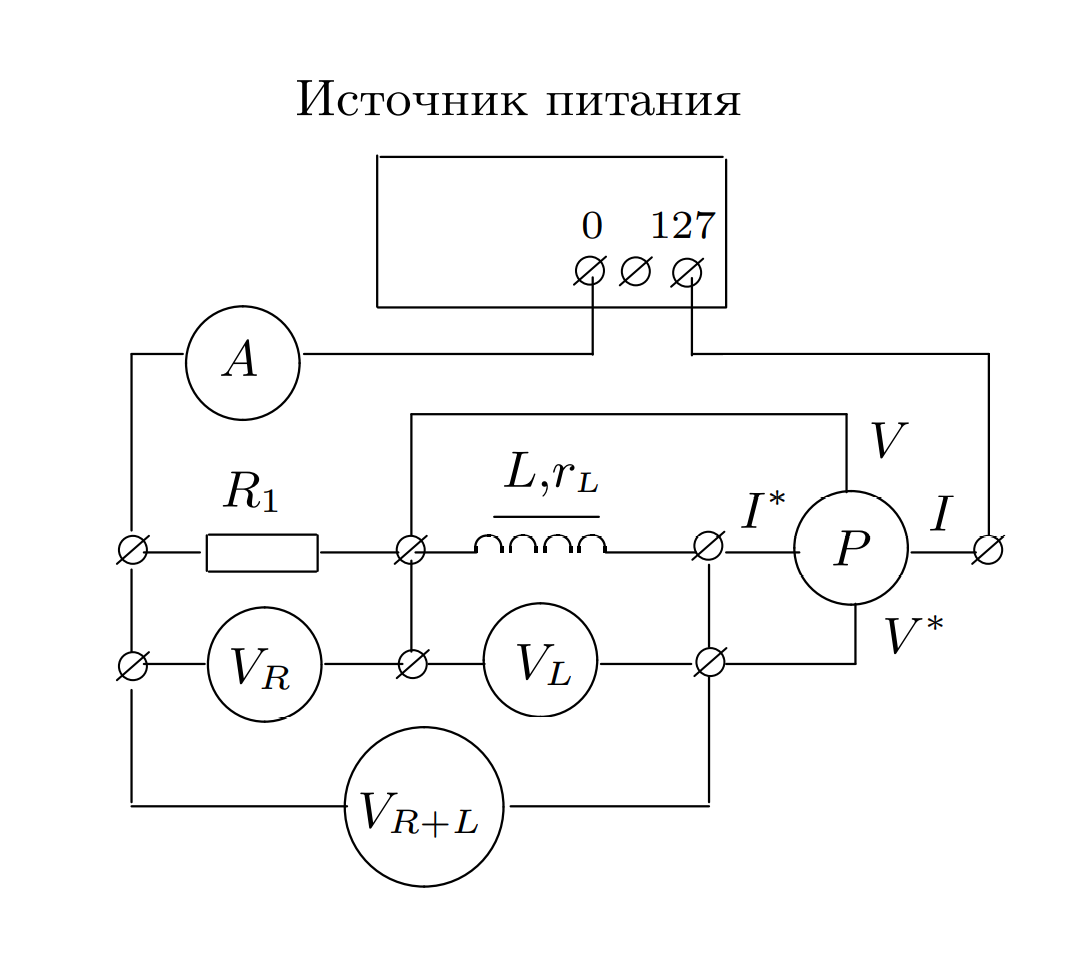
\includegraphics[scale=0.35]{Device}
	\caption{Схема экспериментальной установки} \label{Device}
\end{figure}

Ваттметр электродинамической системы состоит из двух катушек, одна из которых вращается в магнитном поле другой, если через них течёт ток. Токовая катушка ваттметра $II^*$ включается последовательно в исследуемую цепь, а катушка напряжений (потенциальная) $VV^*$ -- параллельно элементу, в котором измеряется выделяемая мощность.

Схема установки для изучения резонанса напряжений изображена на рис. \Ref{Device_2}. Последовательно соединены резистор $R_2\approx5~\Omega$, катушка $L$ и магазин ёмкостей $C$. Амперметр $A$ измеряет ток в цепи, вольтметр $V_C$ -- напряжение на ёмкости, вольтметр $V_{\Sigma}$ -- суммарное напряжение на контуре. Резонанс можно зафиксировать с помощью осциллографа, если подать на вход $X$ напряжение с контура, а на вход $Y$ -- напряжение с резистора $R_2$, пропорциональное току в цепи. В общем случае на экране виден эллипс. При резонансе эллипс вырождается в прямую линию.

\begin{figure}[h]
	\centering
	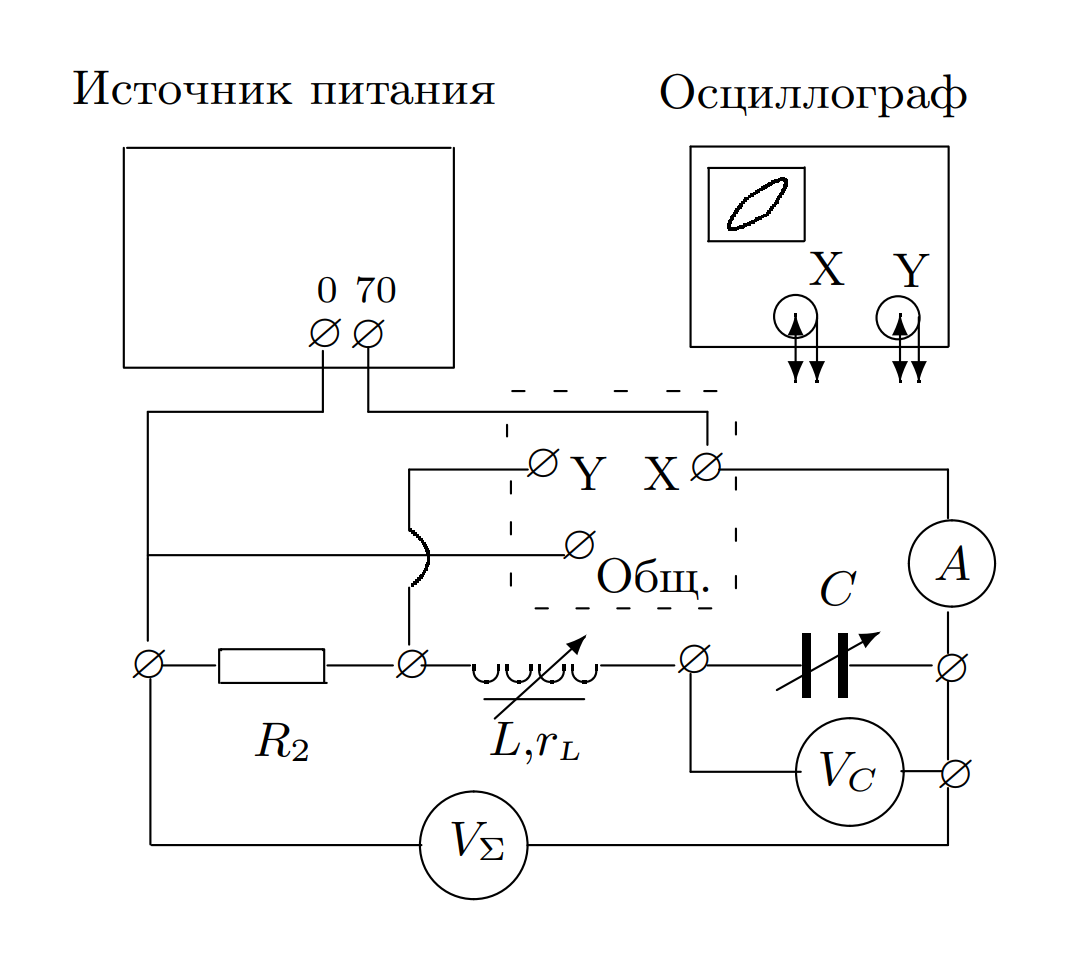
\includegraphics[scale=0.35]{Device_2}
	\caption{Схема экспериментальной установки} \label{Device_2}
\end{figure}

Резонансные напряжения на контуре $U_{\Sigma,\ \text{рез.}}$ и на ёмкости $U_{C,\ \text{рез.}}$ равны соответственно\[U_{\Sigma,\ \text{рез.}}=I_{\text{рез.}}R_{\Sigma},\ U_{C,\ \text{рез.}}=\frac{I_{\text{рез.}}}{\Omega C}.\]Отсюда\[Q=\frac{U_{C,\ \text{рез.}}}{U_{\Sigma,\ \text{рез.}}}.\]Это значит, что добротность контура может быть найдена по измеренным значениям напряжений на контуре и на конденсаторе при резонансе. Зная добротность контура и ёмкость $C$, можно рассчитать $R_{\Sigma}$, а затем определить $r_L$.

\section*{Ход работы}

\subsection*{I. Закон Ома в цепи переменного тока}

Подготовим к работе приборы в схеме, собранной по рис. \Ref{Device}. Подключим в цепь катушку индуктивности, после чего установим на источнике напряжение $U\approx127~\text{В}$. Установим сердечник катушки в положение $x=5~\text{мм}$, после чего запишем показания тока $I$, напряжений $U_R$, $U_L$ и $U_{R+L}$ и мощности $P_L$. Далее будем вытаскивать сердечник из катушки с шагом $\Delta x = 2~\text{мм}$, каждый раз записывая показания всех приборов. Занесём результаты в таблицу \Ref{Ohm}. Среднее положение сердечника $\bar{x}=20~\text{мм}$ также включим в серию измерений.

Также включим в таблицу две колонки для дальнейшей обработки результатов, в одну из которых поместим вычисленные по соответствующей формуле значения $r_L=\frac{P_L}{2I^2}$, а другую -- значения $L=\frac{1}{2\pi\nu_0}\sqrt{\left(\frac{U_L}{I}\right)^2-r_L^2}$, где $\nu_0=50~\text{Гц}$ -- частота сети.

Погрешности приборов составляют половину цены деления шкалы, поэтому $\Delta U=0,5~\text{В}$, а $\Delta I\approx0,01~\text{А}$, $\Delta P\approx0,1~\text{Вт}$, тогда $\sigma_{r_L}=r_L\sqrt{2\left(\frac{\Delta I}{I}\right)^2+\left(\frac{\Delta P_L}{P_L}\right)^2}$ (формулу для $\sigma_L$ здесь приводить не будем в силу её чрезвычайной громоздкости). Занесём эти погрешности в таблицу. Погрешность определения коложения сердечника также составляет половину цены деления и равна $\Delta x=0,5~\text{мм}$.

\begin{table}[h]
	\centering
	\caption{Зависимость тока $I$, напряжений $U_R$, $U_L$ и $U_{R+L}$ и мощности $P_L$ в цепи от положения сердечника $x$} \label{Ohm}
	\begin{tabular}{|c|c|c|c|c|c|c|c|c|c|}
		\hline
		$x$,мм&$I$,А&$U_R$,В&$U_L$,В&$U_{R+L}$,В&$P_L$,Вт&$r_L$,$\Omega$&$L$,мГ&$\sigma_{r_L}$,$\Omega$&$\sigma_L$,мГ\\ \hline
		5 & 0,53 & 42 & 106 & 124 & 16,0 & 28,5 & 610,3 & 1,0 & 13,5 \\ \hline
		7 & 0,60 & 51 & 101 & 123 & 15,3 & 21,3 & 518,5 & 0,7 & 10,4 \\ \hline
		9 & 0,65 & 56 & 97 & 121 & 14,5 & 17,2 & 462,3 & 0,5 & 8,8 \\ \hline
		11 & 0,70 & 60 & 93 & 120 & 14,0 & 14,3 & 413,0 & 0,4 & 7,4 \\ \hline
		13 & 0,73 & 63 & 90 & 119 & 13,5 & 12,7 & 384,1 & 0,4 & 6,7 \\ \hline
		15 & 0,75 & 66 & 87 & 118 & 13,0 & 11,6 & 361,8 & 0,3 & 6,2 \\ \hline
		17 & 0,78 & 68 & 84 & 117 & 12,8 & 10,5 & 336,2 & 0,3 & 5,6 \\ \hline
		19 & 0,80 & 71 & 82 & 117 & 12,5 & 9,8 & 320,3 & 0,3 & 5,2 \\ \hline
		20 & 0,80 & 72 & 81 & 117 & 12,3 & 9,6 & 312,4 & 0,3 & 5,1 \\ \hline
		21 & 0,83 & 73 & 80 & 117 & 12,3 & 9,0 & 301,5 & 0,2 & 4,8 \\ \hline
		23 & 0,85 & 74 & 78 & 116 & 12,3 & 8,5 & 287,1 & 0,2 & 4,5 \\ \hline
		25 & 0,88 & 76 & 76 & 116 & 12,0 & 7,8 & 270,4 & 0,2 & 4,1 \\ \hline
		27 & 0,88 & 77 & 74 & 116 & 12,0 & 7,8 & 263,1 & 0,2 & 4,0 \\ \hline
		29 & 0,90 & 78 & 72 & 115 & 11,8 & 7,3 & 250,4 & 0,2 & 3,8 \\ \hline
		31 & 0,90 & 79 & 71 & 115 & 11,8 & 7,3 & 246,8 & 0,2 & 3,8 \\ \hline
		33 & 0,93 & 80 & 69 & 115 & 11,8 & 6,8 & 232,1 & 0,2 & 3,5 \\ \hline
		35 & 0,93 & 81 & 68 & 114 & 11,5 & 6,7 & 228,9 & 0,2 & 3,4 \\ \hline
		37 & 0,93 & 82 & 67 & 114 & 11,5 & 6,7 & 225,4 & 0,2 & 3,4 \\ \hline
		39 & 0,95 & 82 & 66 & 114 & 11,5 & 6,4 & 217,4 & 0,2 & 3,2 \\ \hline
	\end{tabular}
\end{table}

Использованное в схеме сопротивление $R_1=98~\Omega$. Постром на одном листе графики зависимостей $L$ и $r_L$ от положения сердечника, он приведён на рисунке \Ref{Main_Plot}. Сглаживающие пунктирные кривые получены аппроксимацией экспериментальных точек зависимостью $f\left(x\right)=ax^b$.

\begin{figure}[h]
	\centering
	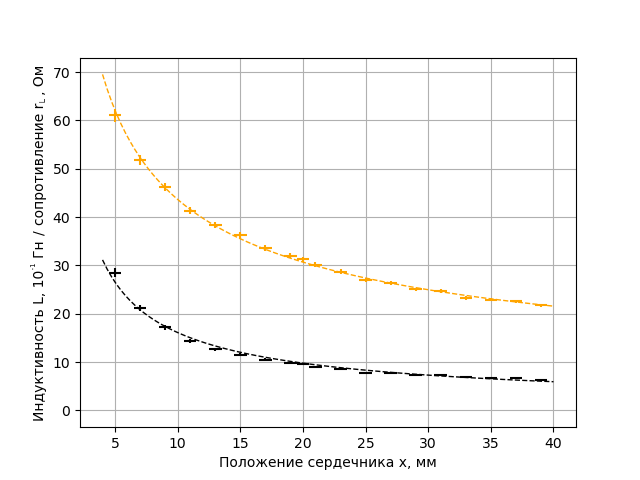
\includegraphics[scale=0.70]{Main_Plot}
	\caption{Зависимость индуктивности $L$ и внутреннего сопротивления катушки $r_L$ от положения сердечника $x$. Сглаживающие кривые проведены по МНК} \label{Main_Plot}
\end{figure}

Из графиков найдём значения $L=\left(295,0\pm5,0\right)~\text{мГн}$ и $r_L=\left(8,6\pm0,3\right)~\Omega$, соответствующие резонансному положению сердечника $x=20~\text{мм}$.

Построим для резонансного положения сердечника векторную диаграмму с горизонтально расположенным $U_R$, приведём её на рисунке \Ref{Diagram}. Отложим на диаграмме активную и реактивную составляющие напряжения на катушке и рассчитаем по ним значения $L$ и $r_L$. Получим $L=\left(295,8\pm5,0\right)~\text{мГн}$ и $r_L=\left(8,5\pm0,3\right)~\Omega$. Определим по диаграмме также косинус сдвига фаз между током и напряжением на катушке, получим $\cos{\theta}=0,177\pm0,007$. Сравним это со значением, рассчитанным с помощью мощности, выделяемой на катушке -- $\cos{\theta}=\frac{P_L}{U_LI}=0,180\pm0,008$.

\begin{figure}[h]
	\centering
	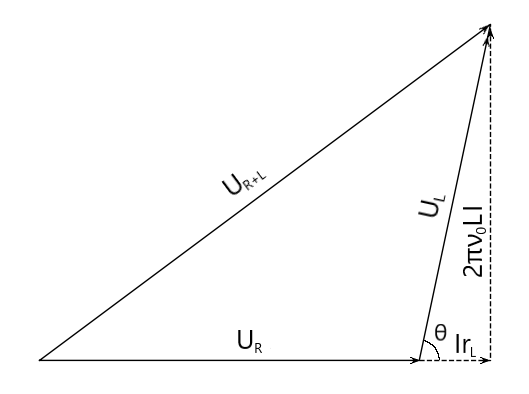
\includegraphics[scale=0.70]{Diagram}
	\caption{Векторная диаграмма для напряжений в схеме} \label{Diagram}
\end{figure}

С помощью теоремы косинусов выразим мощность $P_L$, выделяемую на катушке, через напряжения $U_R$, $U_L$, $U_{R+L}$ и сопротивление $R_1$:\[I=\frac{U_R}{R_1},\\P_L=U_{L,\text{акт}}I,\\U_{L,\text{акт}}=\frac{U_{L+R}^2-U_L^2-U_R^2}{2U_R},\\\implies P_L=\frac{U_{L+R}^2-U_L^2-U_R^2}{2R_1},\]тогда $P_L=\left(11,5\pm0,8\right)~\text{Вт}$ -- видим, что в пределах погрешности полученное значение совпадает с показанием ваттметра.

\subsection*{II. Резонанс напряжений}

Подготовим к работе приборы в схеме, собранной по рис. \Ref{Device_2}. Подберём ёмкость такую, чтобы эллипс на экране электронного осциллографа выродился в прямую, т.е. чтобы контур вошёл в резонанс с частотой сети. Резонансные значения в цепи при этом равны: ток $I=(2,45\pm0,03)~\text{А}$, напряжение на ёмкости $U_{C,\ \text{рез.}}=(256,0\pm1,0)~\text{В}$, а на конденсаторе -- $U_{\Sigma,\ \text{рез.}}=(33,0\pm0,5)~\text{В}$. Отсюда добротность контура можем оценить как\[Q=\frac{U_{C,\ \text{рез.}}}{U_{\Sigma,\ \text{рез.}}}\approx7,76\pm0,15.\]Ёмкость, при которой наступал резонанс, равна $C=31~\text{мкФ}$, координата сердечника при этом $x=(20,0\pm0,5)~\text{мм}$, а величина дополнительного сопротивления $R_2=5,6~\text{мм}$.

Отключим катушку от цепи и при неизменном положении сердечника найдём её омическое сопротивление её витков с помощью омметра и получим величину $r_{L}=(4,53\pm0,02)~\Omega$, а затем найдём с помощью моста переменного тока E7-8 на частотах $50~\text{Гц}$ и $1~\text{кГц}$ значения $L$ и $r_L$: при $50~\text{Гц}$ имеем $L=(291\pm1)~\text{мГн}$ и $r_L=(8,38\pm0,04)~\Omega$, а при $1~\text{кГц}$ -- $L=(250\pm1)~\text{мГн}$ и $r_L=(117\pm1)~\Omega$.

Теперь рассчитаем активное сопротивление катушки $r_L$ через резонансные значения тока и напряжения на контуре по формуле $r_L=\frac{U_{\Sigma,\text{рез}}}{I_{\text{рез}}}-R_2=\left(8,17\pm0,26\right)~\Omega$.

Теперь рассчитаем $L$ и $r_L$ через добротность. Используем формулы $r_L=\frac{1}{Q\Omega C}-R_2=\left(8,23\pm0,15\right)~\Omega$ и $L=\frac{1}{\Omega^2C}=291,8~\text{мГн}$.

Сведём результаты измерений в таблицу \Ref{final}, приведённую ниже.

\begin{table}[h]
	\centering
	\caption{Зависимость тока $I$, напряжений $U_R$, $U_L$ и $U_{R+L}$ и мощности $P_L$ в цепи от положения сердечника $x$} \label{final}
	\begin{tabular}{|c|c|c|c|c|c|c|}
		\hline
		 & Омметр & Мост Е7-8 & График & Вект. диаг & $f\left(I,U_{\Sigma,\text{рез}}\right)$ & $f\left(Q\right)$ \\ \hline
		\hline
		$r_L$, $\Omega$ & 4,53 & 8,38 & 8,60 & 8,50 & 8,17 & 8,23 \\ \hline
		$L$, мГн & -- & 291 & 295,0 & 295,8 & -- & 291,8 \\ \hline
	\end{tabular}
\end{table}

\section*{Вывод}

В данной работе был исследован резонанс напряжений в последовательном колебательном контуре с изменяемой ёмкостью и исследован закон Ома в цепи переменного тока. Результатом подтверждения теоретических предсказаний служит хорошее совпадение параметров катушки -- её индуктивность $L$ и внутреннее сопротивление $r_L$ -- измеренных разными методами. Была также подробно исследована векторная диаграмма контура.

Наиболее точным их них является измерение с помощью моста Е7-8, однако и другие методы можно считать довольно точными, учитывая, что в пределах погрешностей они совпадают с результатами измерений моста (см. таблицу \Ref{final}). Это говорит о корректности проведения эксперимента и правильности работы приборов.

\end{document}
